\documentclass[journal,12pt,onecolumn]{IEEEtran}
\usepackage{cite}
\usepackage{graphicx}
\usepackage{amsmath,amssymb,amsfonts,amsthm}
\usepackage{algorithmic}
\usepackage{graphicx}
\usepackage{textcomp}
\usepackage{xcolor}
\usepackage{txfonts}
\usepackage{listings}
\usepackage{enumitem}
\usepackage{mathtools}
\usepackage{gensymb}
\usepackage{comment}
\usepackage[breaklinks=true]{hyperref}
\usepackage{tkz-euclide} 
\usepackage{listings}
\usepackage{gvv}                                        
%\def\inputGnumericTable{}                                 
\usepackage[latin1]{inputenc} 
\usetikzlibrary{arrows.meta, positioning}
\usepackage{xparse}
\usepackage{color}                                            
\usepackage{array}                                            
\usepackage{longtable}                                       
\usepackage{calc}                                             
\usepackage{multirow}
\usepackage{multicol}
\usepackage{hhline}                                           
\usepackage{ifthen}                                           
\usepackage{lscape}
\usepackage{tabularx}
\usepackage{array}
\usepackage{float}
\newtheorem{theorem}{Theorem}[section]
\newtheorem{problem}{Problem}
\newtheorem{proposition}{Proposition}[section]
\newtheorem{lemma}{Lemma}[section]
\newtheorem{corollary}[theorem]{Corollary}
\newtheorem{example}{Example}[section]
\newtheorem{definition}[problem]{Definition}
\newcommand{\BEQA}{\begin{eqnarray}}
\newcommand{\EEQA}{\end{eqnarray}}
\usepackage{float}
%\newcommand{\define}{\stackrel{\triangle}{=}}
\theoremstyle{remark}
\usepackage{circuitikz}
\usepackage{tikz}

\title{IN  INSTRUMENTATION ENGINEERING}
\author{EE25BTECH11031- Sai Sreevallabh}

\author{Sai Sreevallabh - ee25btech11031}

\begin{document}

\maketitle

\begin{enumerate}

%1
\item If `$\,\rightarrow\,$` denotes increasing order of intensity, then the meaning of the words $[\,\text{drizzle} \rightarrow \text{rain} \rightarrow \text{downpour}\,]$ is analogous to $[\,\rule{1.5cm}{0.4pt} \rightarrow \text{quarrel} \rightarrow \text{feud}\,]$. Which one of the given options is appropriate to fill the blank?
\par\hfill{\brak{\text{GATE IN 2024}}}
    \begin{enumerate}
    \begin{multicols}{4}
    \item bicker
    \item bog
    \item dither
    \item dodge
    \end{multicols}
    \end{enumerate}

%2
\item Statements:

1. All heroes are winners.\\
2. All winners are lucky people.\\
Inferences: \\
I. All lucky people are heroes.\\
II. Some lucky people are heroes.\\
III. Some winners are heroes.\\
Which of the above inferences can be logically deduced from statements 1 and 2?
\par\hfill{\brak{\text{GATE IN 2024}}}
    \begin{enumerate}
        \begin{multicols}{4}
        \item Only I and II
        \item Only II and III
        \item Only I and III
        \item Only III
        \end{multicols}
    \end{enumerate}

%3
\item A student was supposed to multiply a positive real number $p$ with another positive real number $q$. Instead, the student divided $p$ by $q$. If the percentage error in the student's answer is $80\%$, the value of $q$ is
\par\hfill{\brak{\text{GATE IN 2024}}}
    \begin{enumerate}
    \begin{multicols}{4}
    \item $5$
    \item $\sqrt{2}$
    \item $2$
    \item $\sqrt{5}$
    \end{multicols}
    \end{enumerate}

\item If the sum of the first $20$ consecutive positive odd numbers is divided by $20^2$, the result is
\par\hfill{\brak{\text{GATE IN 2024}}}
    \begin{enumerate}
    \begin{multicols}{4}
    \item $1$
    \item $20$
    \item $2$
    \item $\frac{1}{2}$
    \end{multicols}
    \end{enumerate}

%4
\item The ratio of the number of girls to boys in class VIII is the same as the ratio of the number of boys to girls in class IX. The total number of students (boys and girls) in classes VIII and IX is $450$ and $360$, respectively. If the number of girls in classes VIII and IX is the same, then the number of girls in each class is
\par\hfill{\brak{\text{GATE IN 2024}}}
    \begin{enumerate}
    \begin{multicols}{4}
    \item $150$
    \item $200$
    \item $250$
    \item $175$
    \end{multicols}
    \end{enumerate}

\item In the given text, the blanks are (i) - (iv) in their order of occurence. Select the best match for all the blanks.\\
Yoko Roi stands \rule{1.5cm}{0.4pt} as an author for standing \rule{1.5cm}{0.4pt} as an honorary fellow, after she stood \rule{1.5cm}{0.4pt} her writings that stand \rule{1.5cm}{0.4pt} the freedom of speech.
\par\hfill{\brak{\text{GATE IN 2024}}}
    \begin{enumerate}
    \begin{multicols}{4}
    \item 
    \begin{enumerate}
        \item out
        \item down
        \item in
        \item for
    \end{enumerate}
    
    \item 
    \begin{enumerate}
        \item down 
        \item out
        \item by
        \item in
    \end{enumerate}
    
    \item \begin{enumerate}
        \item down 
        \item out
        \item for
        \item in
    \end{enumerate}
    
    \item \begin{enumerate}
        \item out
        \item down
        \item by
        \item for
    \end{enumerate}
    
    \end{multicols}
    \end{enumerate}

%7
\item Seven identical cylindrical chalk-sticks are fitted tightly in a cylindrical container. \figref{7} shows the arrangement of the chalk-sticks inside the cylinder. The length of the container is equal to the length of the chalk-sticks. The ratio of the occupied space to the empty space of the container is
\par\hfill{\brak{\text{GATE IN 2024}}}
\begin{figure}[H]
    \centering
    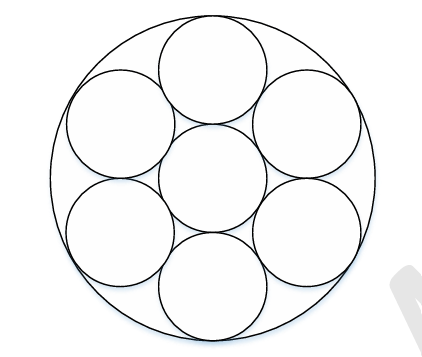
\includegraphics[width=0.3\columnwidth]{Figs/Q-7.png}
    \caption{Chalk-sticks in a container}
    \label{7}
\end{figure}
    \begin{enumerate}
    \begin{multicols}{4}
    \item $\frac{5}{2}$
    \item $\frac{7}{2}$
    \item $\frac{9}{2}$
    \item $3$
    \end{multicols}
    \end{enumerate}

%8
\item The plot in \figref{8} shows the relationship between the mortality risk of cardiovascular disease and the number of steps a person walks per day. Based on the data, which one of the following options is true?
\par\hfill{\brak{\text{GATE IN 2024}}}
\begin{figure}[H]
    \centering
    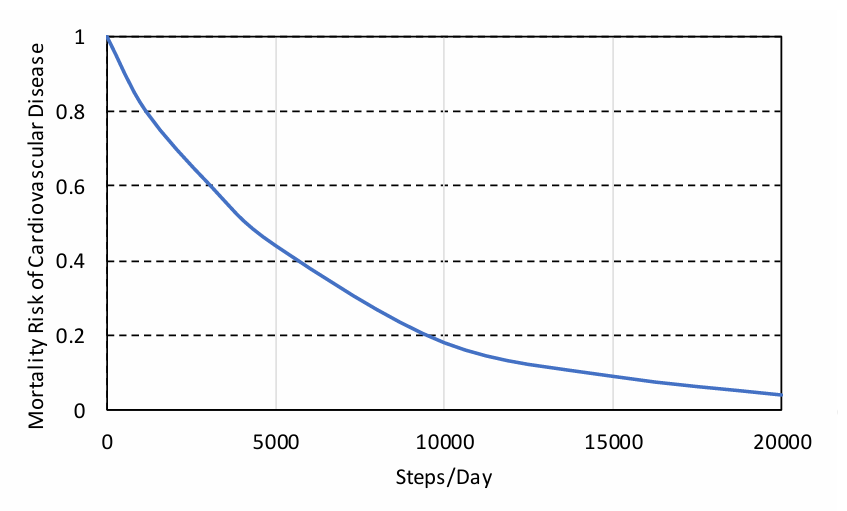
\includegraphics[width=0.5\columnwidth]{Figs/Q-8.png}
    \caption{Graph for Question 8}
    \label{8}
\end{figure}
    \begin{enumerate}
    \begin{multicols}{2}
    \item The risk reduction on increasing the steps/day from $0$ to $10,000$ is less than the risk reduction on increasing the steps/day from $10,000$ to $20,000$.
    \item The risk reduction on increasing the steps/day from $0$ to $5,000$ is less than the risk reduction on increasing the steps/day from $15,000$ to $20,000$.
    \item For any $5,000$ increment in steps/day, the largest risk reduction occurs on going from $0$ to $5,000$.
    \item For any $5,000$ increment in steps/day, the largest risk reduction occurs on going from $15,000$ to $20,000$.
    \end{multicols}
    \end{enumerate}

%9 (((LOTS FOR HEADACHE IMAGES TO PUT)))
\item Five cubes of identical size and another smaller cube are assembled as shown in \figref{9}. If viewed from direction X, the planar image of the assembly appears in \figref{9}. If viewed from direction Y, the planar image of the assembly (in the left of the figure) will appear as
\par\hfill{\brak{\text{GATE IN 2024}}}
\begin{figure}[H]
    \centering
    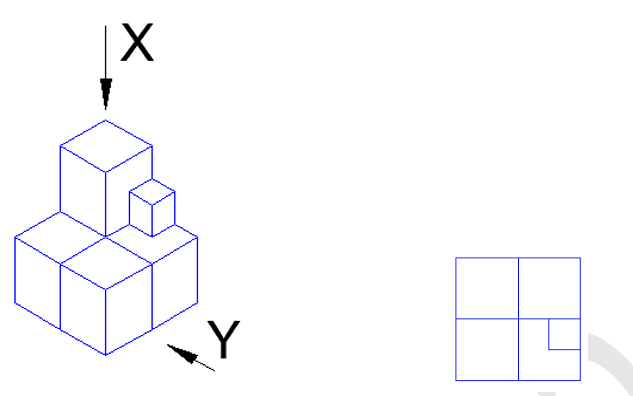
\includegraphics[width=0.5\linewidth]{Figs/Q-9.png}
    \caption{Arrangement of Cubes}
    \label{9}
\end{figure}

    \begin{enumerate}
    \begin{multicols}{2}
    \item 
        \begin{figure}[H]
       % \centering
        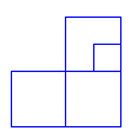
\includegraphics[width=0.3\linewidth]{Figs/Q-9(a).png}
        \end{figure}
        
    \item 
        \begin{figure}[H]
       % \centering
        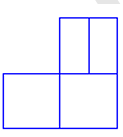
\includegraphics[width=0.3\linewidth]{Figs/Q-9(b).png}
        \end{figure}  
        
    \item 
        \begin{figure}[H]
       % \centering
        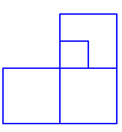
\includegraphics[width=0.3\linewidth]{Figs/Q-9(c).png}
        \end{figure} 

    \item 
        \begin{figure}[H]
        %\centering
        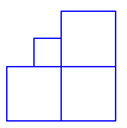
\includegraphics[width=0.3\linewidth]{Figs/Q-9(d).png}
        \end{figure} 

    
    \end{multicols}
    \end{enumerate}

%10
\item Visualize a cube that is held with one of the four body diagonals aligned to the vertical axis. Rotate the cube about this axis such that its view remains unchanged. The magnitude of the minimum angle of rotation is
\par\hfill{\brak{\text{GATE IN 2024}}}
    \begin{enumerate}
    \begin{multicols}{4}
    \item $120\degree$
    \item $60\degree$
    \item $90\degree$
    \item $180\degree$
    \end{multicols}
    \end{enumerate}

%11
\item Let $z = x + i y$ be a complex variable and $\bar{z}$ be its complex conjugate. The equation $\bar{z}^2 + z^2 = 2$ represents a
\par\hfill{\brak{\text{GATE IN 2024}}}
    \begin{enumerate}
    \begin{multicols}{4}
    \item parabola
    \item hyperbola
    \item ellipse
    \item circle
    \end{multicols}
    \end{enumerate}

%12
\item The pressure drop across a control valve is constant. The control valve with inherent characteristic has decreasing sensitivity. If $x$ represents the fraction of maximum stem position of the control valve, then the function $f\brak{x}$ representing the fraction of maximum flow is
\par\hfill{\brak{\text{GATE IN 2024}}}
    \begin{enumerate}
    \begin{multicols}{2}
    \item $\alpha^{x-1}$, where $\alpha$ is constant
    \item $\sqrt{x}$
    \item $x$
    \item $x^2$
    \end{multicols}
    \end{enumerate}

%13
\item A discrete-time sequence is given by $x\sbrak{x} = \sbrak{1,\, 2,\, 3,\,4}$ for $0 \leq n \leq 3$. The zero lag auto-correlation value of $x\sbrak{x}$ is
\par\hfill{\brak{\text{GATE IN 2024}}}
    \begin{enumerate}
    \begin{multicols}{4}
    \item $1$
    \item $10$
    \item $20$
    \item $30$
    \end{multicols}
    \end{enumerate}

%14 ((TABLE TABLE TABLE TABLE))
\item Match the following measuring devices with their principle of measurement.
\begin{table}[H]
    \centering
    \begin{center}
\begin{tabular}{ll}
    \textbf{Group I} & \textbf{Group II} \\
    P. Ferrite & 1. Hexagonal Close Packed (HCP) \\
    Q. Austenite & 2. Body Centered Cubic (BCC) \\
    R. Martensite & 3. Body Centered Tetragonal (BCT) \\
    & 4. Face Centered Cubic (FCC)
\end{tabular}
\end{center} 
\end{table}
\par\hfill{\brak{\text{GATE IN 2024}}}
    \begin{enumerate}
    \begin{multicols}{2}
    \item (P) - (III), (Q) - (IV), (R) - (II), (S) - (I)
    \item (P) - (IV), (Q) - (III), (R) - (II), (S) - (I)
    \item (P) - (III), (Q) - (I), (R) - (IV), (S) - (II)
    \item (P) - (II), (Q) - (IV), (R) - (I), (S) - (III)
    \end{multicols}
    \end{enumerate}

%15
\item The capacitor shown \figref{15} has parallel plates, with each plate having an area $A$. The thickness of the dielectric materials are $d_1$ and $d_2$ and their relative permittivities are $\varepsilon_1$ and $\varepsilon_2$, respectively. Assume that the fringing field effects are negligible and $\varepsilon_0$ is the permittivity of free space.
\begin{figure}[H]
    \centering
    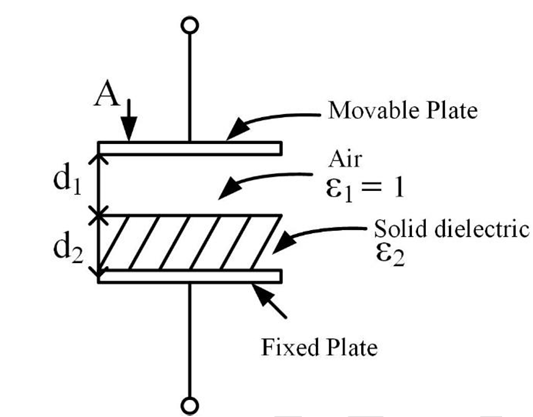
\includegraphics[width=0.5\columnwidth]{Figs/Q-15.png}
    \caption{Parallel Plate Capacitor}
    \label{15}
\end{figure}
If $d_1$ is decreased by $\delta d_1$, the resultant capacitance becomes
\par\hfill{\brak{\text{GATE IN 2024}}}
    \begin{enumerate}
    \begin{multicols}{4}
    \item $\frac{\varepsilon_0 A}{d_1 - \delta d_1 + \frac{d_2}{\varepsilon_2}}$
    \item $\frac{\varepsilon_0 A}{d_2 + {d_1 \over \varepsilon_2}}$
    \item $\frac{\varepsilon_0 A}{d_2 -  \delta d_2 + {d_1 \over \varepsilon_2}}$
    \item $\frac{\varepsilon_0 A}{d_1 + \delta d_1 + {d_2 \over \varepsilon_2}}$
    \end{multicols}
    \end{enumerate}

%16
\item Among the given options, the simplified form of the Boolean function $F = (A+ \bar{A}\cdot B) + \bar{A}\cdot(A+ \bar{B})\cdot C$ is
\par\hfill{\brak{\text{GATE IN 2024}}}
    \begin{enumerate}
    \begin{multicols}{4}
    \item $A + B + C$
    \item $A\cdot B\cdot  C$
    \item $B + \bar{A}\cdot C$
    \item $\bar{A} + B\cdot C$
    \end{multicols}
    \end{enumerate}

%17
\item Consider the state-space representation of a system $$\dot{x} = A x + B u$$ where $x$ is the state vector, $u$ is the input, $A$ is the system matrix and $B$ is the input matrix. Choose the matrix $A$ from the following options such that the system has a pole at the origin.
\par\hfill{\brak{\text{GATE IN 2024}}}
    \begin{enumerate}
    \begin{multicols}{2}
    \item $
    \myvec{
    0 & 1 \\
    -2 & -3
    }$
    
    \item $\myvec{
    1 & -1.5 \\
    -2 & 3
   }$
   
    \item 
    $\myvec{1 & 1.5 \\
    2 & -3}$
    
    \item $
   \myvec{0 & 1 \\
    -2 & 3}
       $
    \end{multicols}
    \end{enumerate}

%18
\item The sinusoidal transfer function corresponding to the polar plot shown in \figref{18}, for $T>0$, is
\par\hfill{\brak{\text{GATE IN 2024}}}
\begin{figure}[H]
    \centering
    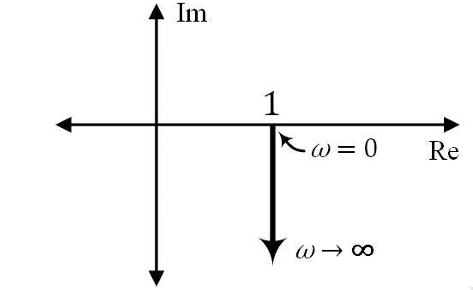
\includegraphics[width=0.4\columnwidth]{Figs/Q-18.png}
    \caption{Polar Plot}
    \label{18}
\end{figure}
    \begin{enumerate}
    \begin{multicols}{4}
    \item $1 - j\omega T$
    \item $\frac{1 - j\omega T}{1 + j\omega T}$
    \item $1 + j\omega T$
    \item $\frac{1}{1 + j\omega T}$
    \end{multicols}
    \end{enumerate}

%19
\item A matrix $M$ is constructed by stacking three column vectors $v_1, v_2, v_3$ as $$M = \myvec{v_1 & v_2 & v_3}$$. Choose the set of vectors from the following options such that $\text{rank}(M) = 3$.
\par\hfill{\brak{\text{GATE IN 2024}}}
    \begin{enumerate}
    \begin{multicols}{2}
    \item $v_1 = \myvec{1\\0\\1},\ v_2 = \myvec{0\\-1\\0},\ v_3 = \myvec{1\\-1\\1}$
    \item $v_1 = \myvec{1\\1\\1},\ v_2 = \myvec{-1\\0\\1},\ v_3 = \myvec{0\\0\\0}$
    \item $v_1 = \myvec{1\\0\\1},\ v_2 = \myvec{-1\\0\\1},\ v_3 = \myvec{1\\-1\\1}$
    \item $v_1 = \myvec{1\\1\\1},\ v_2 = \myvec{-1\\1\\-1},\ v_3 = \myvec{0\\-1\\0}$
    \end{multicols}
    \end{enumerate}

%20
\item The capacitance formed between two concentric spherical metal shells having radii $x$ and $y$ with $y>x$ is ($\epsilon$ is the permittivity of the medium between the shells).
\par\hfill{\brak{\text{GATE IN 2024}}}
    \begin{enumerate}
    \begin{multicols}{4}
    \item $4\pi\epsilon\,\brak{\frac{xy}{y-x}}$
    \item $4\pi\epsilon\,\brak{\frac{x^2}{y-x}}$
    \item $4\pi\epsilon\,\brak{\frac{y^2}{y-x}}$
    \item $4\pi\epsilon\,\brak{\frac{y^2-xy}{x}}$
    \end{multicols}
    \end{enumerate}

%21
\item A linear transducer is calibrated for the ranges shown in \figref{21}. The gain of the transducer is \rule{1.5cm}{0.4pt} mA/$\degree$C (rounded off to two decimal places).
\par\hfill{\brak{\text{GATE IN 2024}}}
\begin{figure}[H]
    \centering
    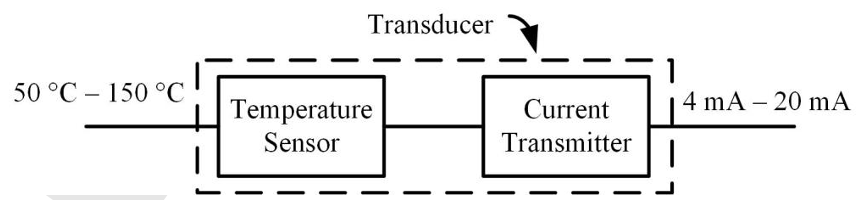
\includegraphics[width=0.5\columnwidth]{Figs/Q-21.png}
    \caption{Linear Transducer}
    \label{21}
\end{figure}

%22
\item Consider a filter defined by the difference equation $y\sbrak{n} - 0.5\,y[n-2] = a\,x\sbrak{n-4}$ where $x\sbrak{n}$ and $y\sbrak{n}$ represent the input and output, respectively. If the magnitude response of the filter at $\omega = \frac{\pi}{2}$ is $|H(\frac{\pi}{2})| = 0.5$, the value of $a$ is \rule{1.5cm}{0.4pt} (rounded off to two decimal places).
\par\hfill{\brak{\text{GATE IN 2024}}}

%23
\item Consider the circuit shown in \figref{23}.\\
\begin{figure}[H]
    \centering
    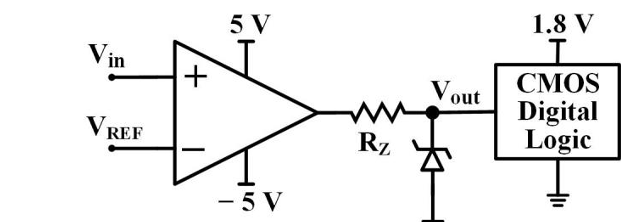
\includegraphics[width=0.5\columnwidth]{Figs/Q-23.png}
    \caption{Circuit Diagram for Question-23}
    \label{23}
\end{figure}
The CMOS digital logic circuit has infinite input impedance. Assume the opamp is ideal. A $1.8$V Zener diode with a minimum Zener current of $2$mA is used. The corresponding maximum value of resistance $R_Z$ is \rule{1.5cm}{0.4pt} k$\ohm$ (rounded off to one decimal place).
\par\hfill{\brak{\text{GATE IN 2024}}}

%24
\item \figref{24} shows an amplifier using an NMOS transistor. Assume that the transistor is in saturation with device parameters, $\mu_n C_{ox} = 250$~$\mu$A/V$^2$, threshold voltage $V_T=0.65$~V and $W/L = 4$. Ignore the channel length modulation effect. The drain current of the transistor at the operating point is \rule{1.5cm}{0.4pt}~$\mu$A (rounded off to nearest integer).
\par\hfill{\brak{\text{GATE IN 2024}}}
\begin{figure}[H]
    \centering
    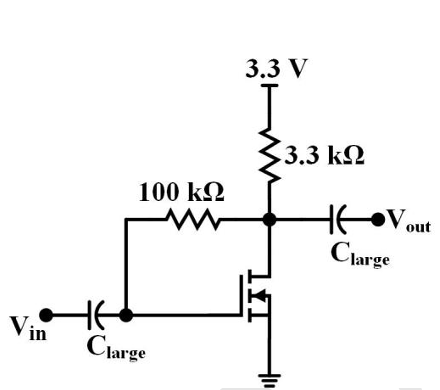
\includegraphics[width=0.5\columnwidth]{Figs/Q-24.png}
    \caption{Amplifier using NMOS Transistor}
    \label{24}
\end{figure}

%25
\item The number of complex multiplications required for computing a $16$-point DFT using the decimation-in-time radix-$2$ FFT is \rule{1.5cm}{0.4pt} (in integer).
\par\hfill{\brak{\text{GATE IN 2024}}}

%26
\item A $3\times 3$ matrix $P$ with all real elements has eigenvalues $\frac{1}{4}$, $1$, and $-2$. The value of $\abs{P^{-1}}$ is \rule{1.5cm}{0.4pt} (rounded off to nearest integer).
\par\hfill{\brak{\text{GATE IN 2024}}}

%27
\item The Nyquist sampling frequency for $x\brak{t} = 10\sin^2(200\pi t)$ is \rule{1.5cm}{0.4pt} Hz (rounded off to nearest integer).
\par\hfill{\brak{\text{GATE IN 2024}}}

%28
\item The resistance of a $20$~k$\ohm$ resistor is measured six consecutive times using an LCR meter. The first five readings are $19$~k$\ohm$, $18$~k$\ohm$, $23$~k$\ohm$, $21$~k$\ohm$ and $17$~k$\ohm$.\\
If the mean of the measurements and the true value are equal, the last reading is \rule{1.5cm}{0.4pt}~k$\ohm$ (rounded off to nearest integer).
\par\hfill{\brak{\text{GATE IN 2024}}}

%29
\item Consider the readout circuit of a piezoelectric sensor shown \figref{29}.\\
When the piezoelectric sensor generates a charge $q_p$, the resulting change in voltage $V_x$ is $-2$~V. Then the corresponding change in the voltage $V_{out}$ is \rule{1.5cm}{0.4pt}~V (rounded off to nearest integer).\\Note: Assume all components are ideal.
\par\hfill{\brak{\text{GATE IN 2024}}}
\begin{figure}[H]
    \centering
    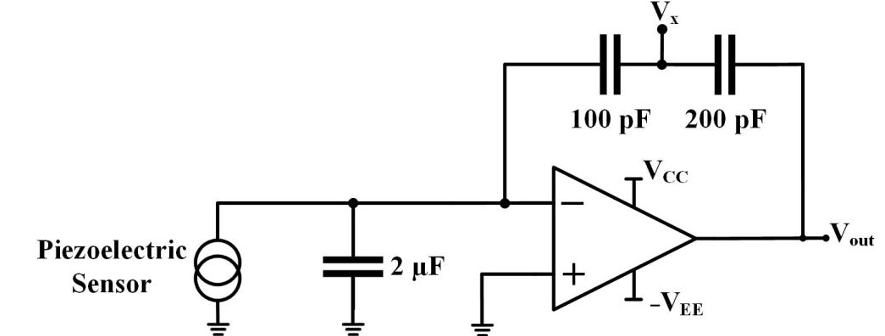
\includegraphics[width=0.5\columnwidth]{Figs/Q-29.png}
    \caption{Readout Circuit of a Piezoelectric Sensor}
    \label{29}
\end{figure}

\item The voltage applied and the current drawn by a circuit are\\
 $$v\brak{t} = 95 + 200\cos(120\pi t) + 90\cos(360\pi t - 60\degree)\ \text{V}$$
$$i\brak{t} = 4\cos(120\pi t - 60\degree) + 1.5\cos(240\pi t - 75\degree) \ \text{A}$$   
The average power absorbed by the circuit is \rule{1.5cm}{0.4pt}~W (rounded off to nearest integer).
\par\hfill{\brak{\text{GATE IN 2024}}}

%31
\item The current $i\brak{t}$ drawn by a circuit is given as\\
$i\brak{t} = 4 + 30\cos\brak{t} - 20\sin\brak{t} + 15\cos(3t) - 10\sin(3t)\ \text{A}$\\
The root-mean-square value of $i\brak{t}$ is \rule{1.5cm}{0.4pt}~A (rounded off to one decimal place).
\par\hfill{\brak{\text{GATE IN 2024}}}

%32
\item A linear potentiometer ($0-10$~k$\ohm$) is used to measure the water level as shown in \figref{32}. The resistance between $A$ and $C$ varies linearly from $0$ to $10$~k$\ohm$ for a change in water level from $0$ to $20$cm. The sensor is excited using a DC voltage source, $V_S = 10$~V with an internal resistance, $R_S = 200~\ohm$. If $V_{out} = 5$~V, the water level is \rule{1.5cm}{0.4pt}~cm (rounded off to one decimal place).
\par\hfill{\brak{\text{GATE IN 2024}}}
\begin{figure}[H]
    \centering
    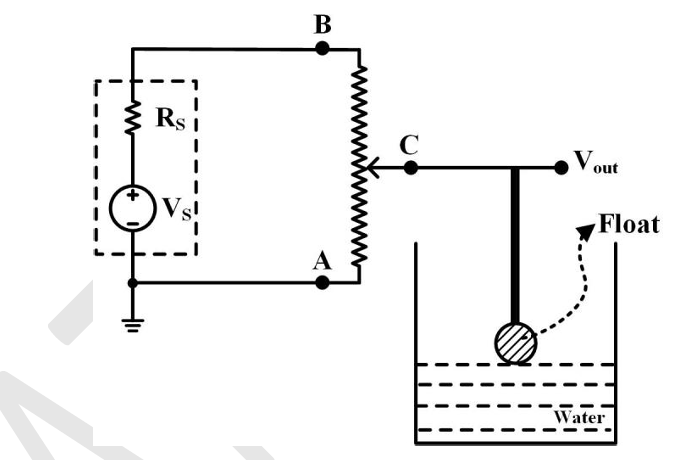
\includegraphics[width=0.4\columnwidth]{Figs/Q-32.png}
    \caption{Diagram for Question-32}
    \label{32}
\end{figure}

%33
\item The switch in \figref{33} has been closed for a long time ($t<0$). It is opened at $t=0$~seconds. The value of $\frac{d v_c}{dt}$ at $t=0^+$ is \rule{1.5cm}{0.4pt}~V/s (rounded off to nearest integer).
\par\hfill{\brak{\text{GATE IN 2024}}}
\begin{figure}[H]
    \centering
    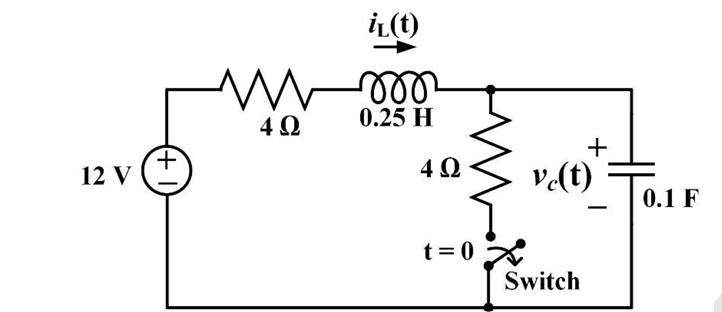
\includegraphics[width=0.5\columnwidth]{Figs/Q-33.png}
    \caption{Circuit Diagram for Question-33}
    \label{33}
\end{figure}

%34
\item Consider a system given by the following first order differential equation:
$$\frac{dy}{dt} = y + 2t - t^2$$
where, $y\brak{0}=1$ and $0\leq t < \infty$. Using a step size $h=0.1$ for the improved Euler method, the value of $y\brak{t}$ at $t=0.1$ is \rule{1.5cm}{0.4pt} (rounded off to two decimal places).
\par\hfill{\brak{\text{GATE IN 2024}}}

%25
\item Indian Premier League has divided the sixteen cricket teams into two equal pools: Pool-A and Pool-B. Four teams of Pool-A have blue logo jerseys while the rest four have red logo jerseys. Five teams of Pool-B have blue logo jerseys while the rest three have red logo jerseys.\\
If one team from each pool reaches the final, the probability that one team has a blue logo jersey and another has a red logo jersey is \rule{1.5cm}{0.4pt} (rounded off to one decimal place).
\par\hfill{\brak{\text{GATE IN 2024}}}

%36
\item A wire of circular cross section with radius $a$ is shown in \figref{36}. The current density is given by $J = k s^2$, where $k$ is a constant, $s$ is the radial distance from the axis and $0 \leq s \leq a$. The total current $I$ in the wire is
\par\hfill{\brak{\text{GATE IN 2024}}}
\begin{figure}[H]
    \centering
    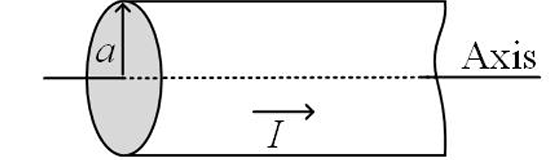
\includegraphics[width=0.4\columnwidth]{Figs/Q-36.png}
    \caption{Wire of Circular Cross Section}
    \label{36}
\end{figure}
    \begin{enumerate}
    \begin{multicols}{4}
    \item $\frac{\pi k a^4}{2}$
    \item $\frac{2\pi k a^3}{3}$
    \item $\frac{\pi k a^3}{2}$
    \item $\frac{\pi k a^4}{4}$
    \end{multicols}
    \end{enumerate}

%37
\item The measured values from a flow instrument, whose range is between $0$ and $2$ flow units, are shown in the histogram in \figref{37}. The systematic error (bias) and the maximum error (in flow units), respectively are
\par\hfill{\brak{\text{GATE IN 2024}}}
\begin{figure}[H]
    \centering
    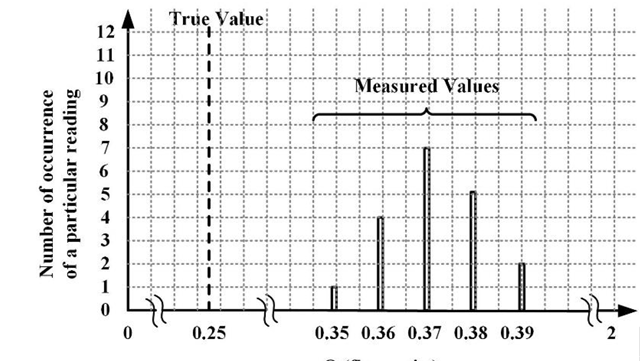
\includegraphics[width=0.6\columnwidth]{Figs/Q-37.png}
    \caption{Histogram for Question-37}
    \label{37}
\end{figure}
    \begin{enumerate}
    \begin{multicols}{4}
    \item $0.12$ and $0.14$
    \item $0.01$ and $0.10$
    \item $0.10$ and $0.14$
    \item $0.04$ and $0.12$
    \end{multicols}
    \end{enumerate}

%38
\item Consider a discrete-time sequence
$$x\sbrak{n}=
\begin{cases}
(0.2)^n,& 0 \leq n \leq 7, \\
0 &\text{otherwise}
\end{cases}$$.
The region of convergence of $X\brak{z}$, the $z$-transform of $x\sbrak{n}$, consists of
\par\hfill{\brak{\text{GATE IN 2024}}}
    \begin{enumerate}
    \begin{multicols}{2}
    \item all values of $z$ except $z=0.2$
    \item all values of $z$
    \item all values of $z$ except $z=0$
    \item all values of $z$ except $z=\infty$
    \end{multicols}
    \end{enumerate}

%39
\item In the bridge circuit shown in \figref{39}, under balanced condition, the values of $R$ and $C$ respectively, are
\par\hfill{\brak{\text{GATE IN 2024}}}
\begin{figure}[H]
    \centering
    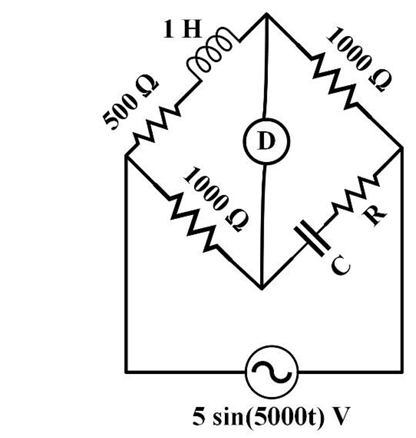
\includegraphics[width=0.3\columnwidth]{Figs/Q-39.png}
    \caption{Bridge Circuit}
    \label{39}
\end{figure}
    \begin{enumerate}
    \begin{multicols}{2}
    \item $1.010\,\ohm$ and $19.802\,\mu\mathrm{F}$
    \item $9.901\,\ohm$ and $0.505\,\mu\mathrm{F}$
    \item $19.802\,\ohm$ and $1.01\,\mu\mathrm{F}$
    \item $39.604\,\ohm$ and $2.02\,\mu\mathrm{F}$
    \end{multicols}
    \end{enumerate}

\item Laplace transform of a signal $x\brak{t}$ is $$X(s) = \frac{1}{s^2 + 13s + 42}$$\\
Let $u\brak{t}$ be the unit step function. Choose the signal $x\brak{t}$ from the following options if the region of convergence is $-7 < Re\cbrak{s} < -6$.
\par\hfill{\brak{\text{GATE IN 2024}}}
    \begin{enumerate}
    \begin{multicols}{2}
    \item $-e^{-6t}u\brak{t} - e^{-7t}u(-t)$
    \item $-e^{-6t}u(-t) - e^{-7t}u\brak{t}$
    \item $e^{-6t}u\brak{t} - e^{-7t}u(-t)$
    \item $-e^{-6t}u(-t) - e^{-7t}u(-t)$
    \end{multicols}
    \end{enumerate}


%41
\item In \figref{41}, both the opamps $A_1$ and $A_2$ are ideal, except that the opamp $A_1$ has an offset voltage $(V_{os})$ of $1$~mV. For $V_{in} = 0$~V, the values of the output voltages $V_{out1}$ and $V_{out2}$, respectively, are
\par\hfill{\brak{\text{GATE IN 2024}}}
\begin{figure}[H]
    \centering
    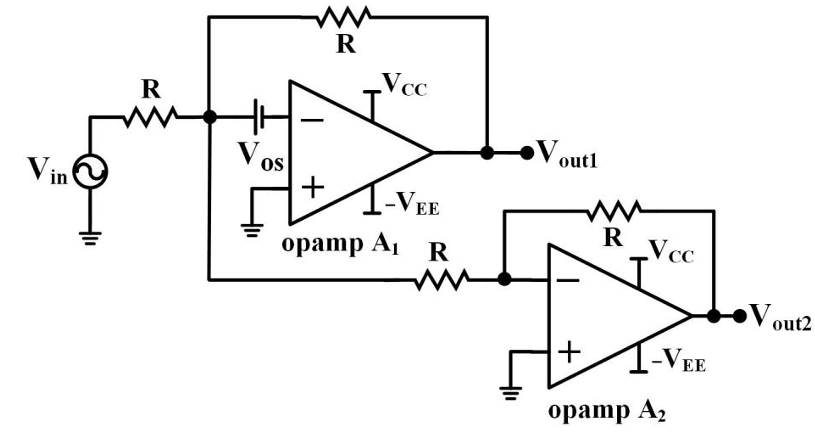
\includegraphics[width=0.5\columnwidth]{Figs/Q-41.png}
    \caption{Circuit Diagram for Question-41}
    \label{41}
\end{figure}
    \begin{enumerate}
    \begin{multicols}{4}
    \item $3$~mV and $-1$~mV
    \item $1$~mV and $0$~mV
    \item $1$~mV and $-1$~mV
    \item $2$~mV and $0$~mV
    \end{multicols}
    \end{enumerate}

%42
\item In \figref{42}, the positive edge triggered D flip-flops are initially reset to $Q=0$. The logic gates and the multiplexers have no propagation delay. After reset, a train of clock pulses (CLK) are applied. The logic-states of the inputs DIN, S and the clock pulses are also shown in the figure. Assuming no timing violations, the sequence of output $Y$ from the $3$rd clock to the $5$th clock, $Y_3 Y_4 Y_5$ is
\par\hfill{\brak{\text{GATE IN 2024}}}
\begin{figure}[H]
    \centering
    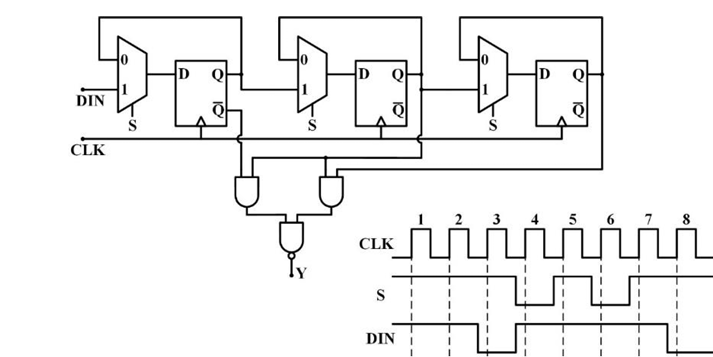
\includegraphics[width=0.5\columnwidth]{Figs/Q-42.png}
    \caption{Circuit Diagram for Question 42}
    \label{42}
\end{figure}
    \begin{enumerate}
    \begin{multicols}{4}
    \item 001
    \item 010
    \item 000
    \item 011
    \end{multicols}
    \end{enumerate}

%43
\item In \figref{43}, $R = 1$~k$\ohm$ and $C=0.1~\mu$F. For a dc gain of $-10$, the $3$~dB cut-off frequency (rounded off to one decimal place) is\\
Assume the opamp is ideal.
\par\hfill{\brak{\text{GATE IN 2024}}}
\begin{figure}[H]
    \centering
    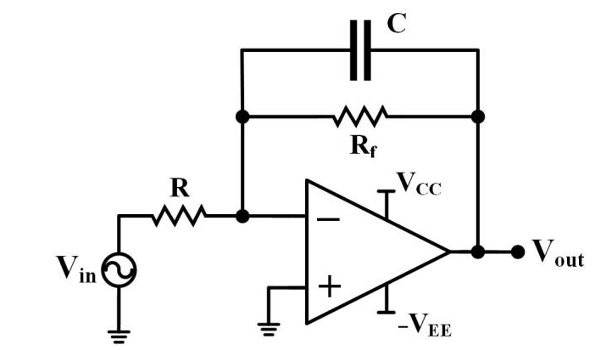
\includegraphics[width=0.5\columnwidth]{Figs/Q-43.png}
    \caption{Circuit Diagram for Question 43}
    \label{43}
\end{figure}
    \begin{enumerate}
    \begin{multicols}{4}
    \item $159.1$~Hz
    \item $1591.5$~Hz
    \item $1750.7$~Hz
    \item $175.0$~Hz
    \end{multicols}
    \end{enumerate}

%44
\item Consider the feedback control system shown in \figref{44}. The steady-state error 
$e_{ss} = \lim_{t \to \infty} \brak{r\brak{t} - y\brak{t}}$ due to unit step reference $r\brak{t}$ is
\par\hfill{\brak{\text{GATE IN 2024}}}
\begin{figure}[H]
    \centering
    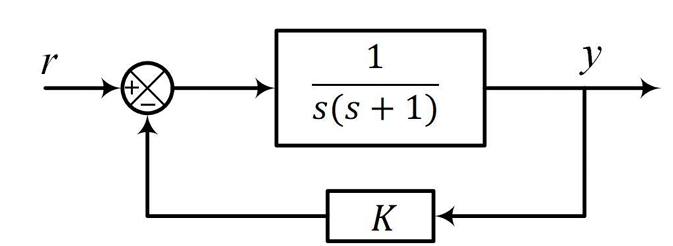
\includegraphics[width=0.5\columnwidth]{Figs/Q-44.png}
    \caption{Feedback Control System}
    \label{44}
\end{figure}
    \begin{enumerate}
    \begin{multicols}{4}
    \item $\frac{K-1}{K}$
    \item $\frac{1}{2}$
    \item $0$
    \item$\frac{1-K}{K}$
    \end{multicols}
    \end{enumerate}

%45
\item The transfer function of a system is 
$$G(s) = \frac{\omega_n^2}{s^2 + 2 \xi \omega_n s + \omega_n^2}$$
Choose the range of $\xi$ and $\omega_n$ (in rad/s) from the following options such that the poles lie on the shaded region of the $s$-plane as shown in \figref{45}.
\par\hfill{\brak{\text{GATE IN 2024}}}
\begin{figure}[H]
    \centering
    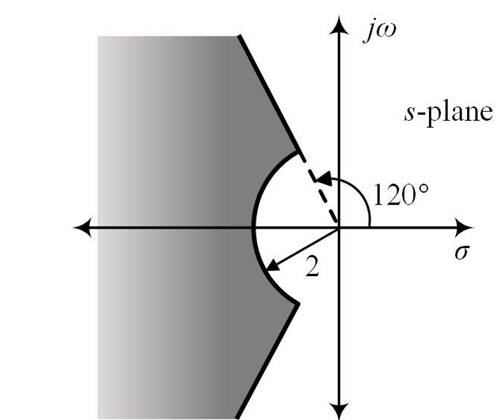
\includegraphics[width=0.4\columnwidth]{Figs/Q-45.png}
    \caption{Diagram for Question-45}
    \label{45}
\end{figure}
    \begin{enumerate}
    \begin{multicols}{4}
    \item $\xi \geq \frac{1}{2}$ and $\omega_n \geq 2$
    \item $\xi \geq \frac{1}{4}$ and $\omega_n \geq 2$
    \item $\xi \geq \frac{1}{2}$ and $\omega_n \geq \sqrt{3}$
    \item $\xi \geq \frac{1}{4}$ and $\omega_n \geq \sqrt{3}$
    \end{multicols}
    \end{enumerate}

%46
\item Let $C$ be the closed curve in the $xy$-plane, traversed in the counterclockwise direction along the boundary of the rectangle with vertices at $(0,0), (2,0), (2,1), (0,1)$. The value of the line integral
$$
\oint_C \brak{-e^y \, dx + e^x \, dy}
$$
is 
\par\hfill{\brak{\text{GATE IN 2024}}}
    \begin{enumerate}
    \begin{multicols}{4}
    \item $e^2 + 2 e -3$
    \item $e^2 - 2e -3$
    \item $e^2 + e - 1$
    \item $e^2 + e + 1$
    \end{multicols}
    \end{enumerate}

%47
\item In \figref{47}, assume  
\begin{itemize}
    \item $\alpha$ is the phase angle between the load current and the load voltage,
    \item $\beta$ is the phase angle by which pressure coil current lags the pressure coil voltage of the wattmeter,
    \item $\gamma$ is the phase angle between currents in the pressure coil and the current coil of the wattmeter,
    \item $\delta$ is the phase angle of the voltage transformer,
    \item $\theta$ is the phase angle of the current transformer.
\end{itemize}
When the load has a lagging phase angle of $\alpha$, which one of the following options is correct?
\par\hfill{\brak{\text{GATE IN 2024}}}
\begin{figure}[H]
    \centering
    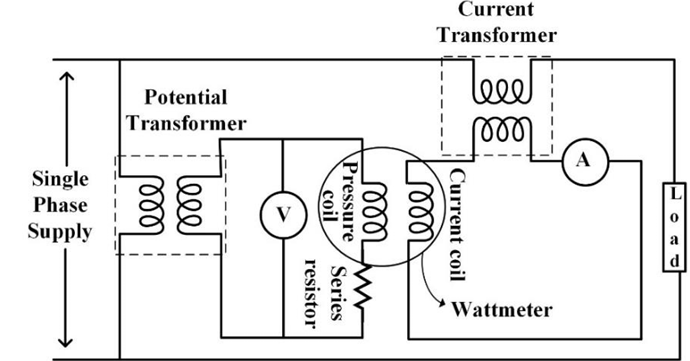
\includegraphics[width=0.5\columnwidth]{Figs/Q-47.png}
    \caption{Diagram for Question-47}
    \label{47}
\end{figure}
    \begin{enumerate}
    \begin{multicols}{4}
    \item $\alpha = -\gamma \pm \delta \pm \theta - \beta$
    \item $\alpha = -\gamma \pm \delta \pm \theta + \beta$
    \item $\alpha = \gamma \pm \delta \pm \theta + \beta$
    \item $\alpha = \gamma \pm \delta \pm \theta - \beta$
    \end{multicols}
    \end{enumerate}

%48
\item Consider an ultrasonic measurement system shown in the figure. The ultrasonic transmitter \brak{t} sends a continuous wave signal $x\brak{t} = \cos(2 \pi f_1 t)$ volts towards an object whose vibration is modeled as $m\brak{t} = 0.5 \sin(2 \pi f_2 t)$ volts. Neglecting the phase shift due to any other effect, the received signal at the receiver (R) is
\[
y\brak{t} = \cos \left( 2 \pi f_1 t + \beta \cos (2 \pi f_2 t) \right) \text{ volts}.
\]
Assuming the frequency sensitivity factor as 500 Hz/volt, $f_1 = 40$ kHz, $f_2 = 1$ kHz, the modulation index $(\beta)$ and the frequency deviation in $y\brak{t}$, respectively, are
\par\hfill{\brak{\text{GATE IN 2024}}}
\begin{figure}[H]
    \centering
    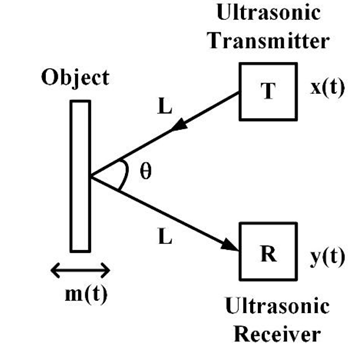
\includegraphics[width=0.3\columnwidth]{Figs/Q-48.png}
    \caption{Ultrasonic Measurement System}
    \label{48}
\end{figure}
    \begin{enumerate}
    \begin{multicols}{4}
    \item $0.25$ and $\pm 250$ Hz
    \item $0.5$ and $\pm 500$ Hz
    \item $1$ and $\pm 1000$ Hz
    \item $0.75$ and $\pm 1000$ Hz
    \end{multicols}
    \end{enumerate}

%49
\item The complex functions $f(z) = u(x,y) + i \, v(x,y)$ and $\bar{f}(z) = u(x,y) - i v(x,y)$ are both analytic in a given domain. Choose the correct option(s) from the following.
\par\hfill{\brak{\text{GATE IN 2024}}}
    \begin{enumerate}
    \begin{multicols}{4}
    \item $\frac{\partial u}{\partial x} = \frac{\partial v}{\partial y} = 0$
    \item $\frac{\partial u}{\partial y} = - \frac{\partial v}{\partial x} \neq 0$
    \item $\frac{df(z)}{dz} = 0$
    \item $\frac{df(z)}{dz} \neq 0$
    \end{multicols}
    \end{enumerate}

%50 
\item The readings recorded from a 20-psig pressure gauge are given in the Table. The regression line obtained for the data is $y = 0.04 x + 10.32$. The regression coefficient of determination, $R^2 =$ \rule{1.5cm}{0.4pt} (rounded off to three decimal places).

\begin{table}[H]
\centering
\begin{tabular}{|c|c|c|}
     \hline
     \textbf{Mineral} & \textbf{Modal abundance \brak{\%}} & \textbf{Partition coefficient}\\
     \hline
     Clinopyroxene & $45$ & $0.506$ \\
      \hline
      Orthopyroxene & $40$ & $0.42$ \\
      \hline
      Olivine & $10$ & $0.045$ \\
      \hline
      Plagioclase & $05$ & $0.019$ \\
      \hline
\end{tabular}
\end{table}

%51
\item In \figref{51}, $R = 4.5$ k$\ohm$, $\Delta R = 1.5$ k$\ohm$, and INA is assumed to be ideal. The equivalent resistance between A and B is \rule{1.5cm}{0.4pt} k$\ohm$ (rounded off to nearest integer).
\par\hfill{\brak{\text{GATE IN 2024}}}
\begin{figure}[H]
    \centering
    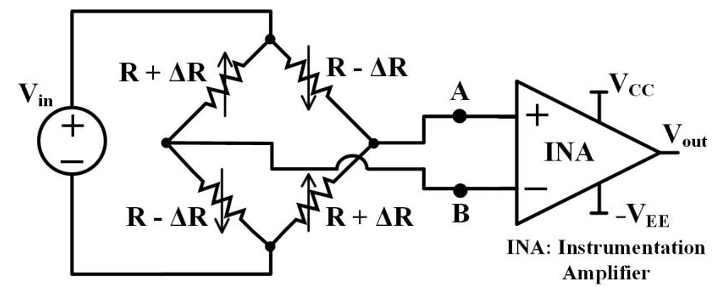
\includegraphics[width=0.4\columnwidth]{Figs/Q-51.png}
    \caption{Diagram for Question-51}
    \label{51}
\end{figure}

%52
\item Consider the capacitive sensor circuit and its output voltage shown in \figref{52}. The circuit is switched ON at $t=0$. Assuming the opamp to be ideal, the frequency of the output voltage $V_o$ is \rule{1.5cm}{0.4pt} kHz (rounded off to two decimal places).
\par\hfill{\brak{\text{GATE IN 2024}}}
\begin{figure}[H]
    \centering
    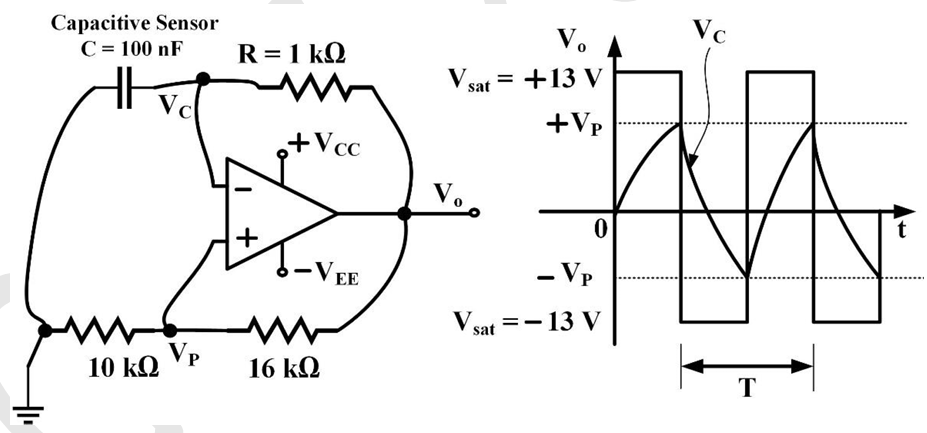
\includegraphics[width=0.7\columnwidth]{Figs/Q-52.png}
    \caption{Diagram for Question-52}
    \label{52}
\end{figure}

%53
\item The $4$-point DFTs of two sequences $x\sbrak{n}$ and $y\sbrak{n}$ are $X[k] = [1, -j, 1, j]$ and $Y[k] = [1, 3j, 1, -3j]$, respectively. Assuming $z\sbrak{n}$ represents the $4$-point circular convolution of $x\sbrak{n}$ and $y\sbrak{n}$, the value of $z\sbrak{0}$ is \rule{1.5cm}{0.4pt} (rounded off to nearest integer).

Note: The DFT of an $N$-point sequence $x\sbrak{n}$ is defined as 
$$
X\sbrak{k} = \sum_{n=0}^{N-1} x\sbrak{n} e^{\frac{-j 2\pi n k}{N}}.
$$
\par\hfill{\brak{\text{GATE IN 2024}}}

%54
\item Consider \figref{54}. For zero deflection in the galvanometer, the required value of resistor $R_x$ is \rule{1.5cm}{0.4pt} $\ohm$ (rounded off to nearest integer).
\par\hfill{\brak{\text{GATE IN 2024}}}
\begin{figure}[H]
    \centering
    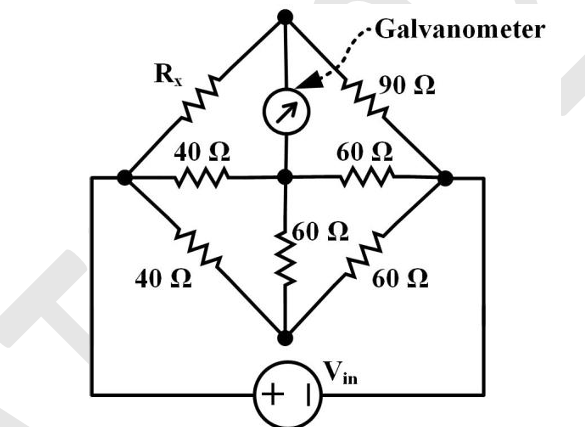
\includegraphics[width=0.4\columnwidth]{Figs/Q-54.png}
    \caption{Diagram for Question-54}
    \label{54}
\end{figure}

%55
\item Consider a unity negative feedback system with its open-loop pole-zero map as shown in \figref{55}. If the point $s = j \alpha$, $\alpha >0$, lies on the root locus, the value of $\alpha$ is \rule{1.5cm}{0.4pt} (rounded off to nearest integer). Note: The poles are marked with $\times$ in the figure.
\par\hfill{\brak{\text{GATE IN 2024}}}
\begin{figure}[H]
    \centering
    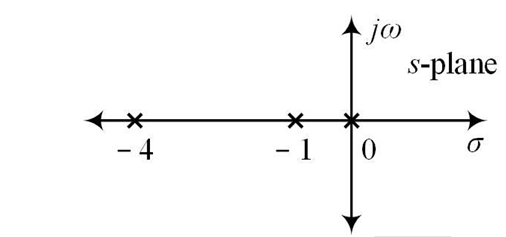
\includegraphics[width=0.4\columnwidth]{Figs/Q-55.png}
    \caption{Open-Loop Pole-Zero map}
    \label{55}
\end{figure}

%56
\item A shielded cable with $C_{stray} = 20$ pF and $R_{wire} = 10~\ohm$ is used to connect the inductive sensors as shown in the figure. The RMS value of $V_{out}$ is \rule{1.5cm}{0.4pt} V (rounded off to two decimal places). Note: Assume all components are ideal, and sensors are not magnetically coupled.
\par\hfill{\brak{\text{GATE IN 2024}}}

%57
\item In \figref{57}, the diode current is given by $I_D = I_S e^{\alpha V_D / T}$. $V_D$ is the diode voltage in volts, $T$ is the absolute temperature in Kelvin, $\alpha=1.16 \times 10^{4}$ K/V, and $I_S = 10^{-15}$ A is the saturation current. The dc current source, opamp and the resistors are ideal, and are assumed to be temperature independent. The change in the output voltage ($V_{out}$) per Kelvin change in temperature is \rule{1.5cm}{0.4pt} mV (rounded off to one decimal place).
\par\hfill{\brak{\text{GATE IN 2024}}}
\begin{figure}[H]
    \centering
    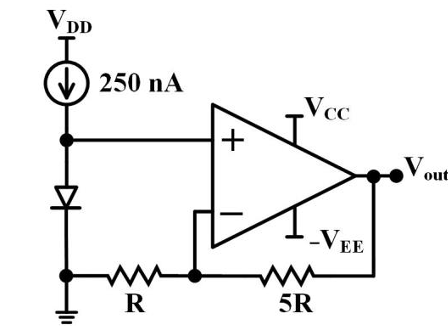
\includegraphics[width=0.3\columnwidth]{Figs/Q-57.png}
    \caption{Diagram for Question-57}
    \label{57}
\end{figure}

%58
\item An ADC has a full scale voltage of $1.4$ V, resolution of $200$ mV, and produces binary output data. The input signal of the ADC has a bandwidth of $500$ MHz, and it samples the data at the Nyquist rate. The parallel data output is converted to a serial bit stream using a parallel-to-serial converter. The data rate at the output of the parallel-to-serial converter is \rule{1.5cm}{0.4pt} Gbps (rounded off to nearest integer).
\par\hfill{\brak{\text{GATE IN 2024}}}

%59
\item In the circuit shown in \figref{59}, assume the opamp is ideal and the initial charge on the capacitor is zero. The output voltage at time $t=2$ ms is \rule{1.5cm}{0.4pt} V (rounded off to one decimal place).
\par\hfill{\brak{\text{GATE IN 2024}}}
\begin{figure}[H]
    \centering
    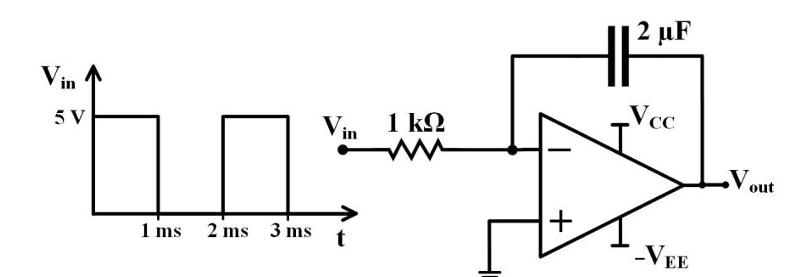
\includegraphics[width=0.4\columnwidth]{Figs/Q-59.png}
    \caption{Diagram for Question-59}
    \label{59}
\end{figure}

%60
\item In \figref{60}, SW is a switch whose position changes from $1$ to $0$ when $V_C$ changes from logic HIGH to LOW and vice versa. The bandwidth of the permanent magnet moving coil (PMMC) type voltmeter is $1$ Hz. If $V_{sense} = 2 \sin(4000 \pi t)$ V and $V_{ref} = 4 \sin(2000 \pi t)$ V, the voltmeter reading is \rule{1.5cm}{0.4pt} V (rounded off to nearest integer).\\
Note: Assume all components are ideal.
\par\hfill{\brak{\text{GATE IN 2024}}}
\begin{figure}[H]
    \centering
    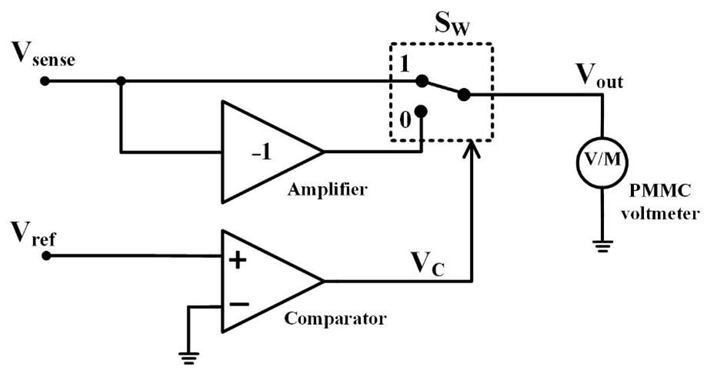
\includegraphics[width=0.4\columnwidth]{Figs/Q-60.png}
    \caption{Diagram for Question-60}
    \label{60}
\end{figure}

%61
\item A $50\text{kVA}$ transformer has an efficiency of $95\%$ at full load and unity power factor. Assume the core losses are negligible. The efficiency of the transformer at $75\%$ of the full load and $0.8$ power factor is \rule{1.5cm}{0.4pt}\% (rounded off to one decimal place).
\par\hfill{\brak{\text{GATE IN 2024}}}

%62
\item A three-phase squirrel-cage induction motor has a starting torque of $100\%$ of the full load torque and a maximum torque of $300\%$ of the full load torque. Neglecting the stator impedance, the slip at the maximum torque is \rule{1.5cm}{0.4pt}\% (rounded off to two decimal places). \par\hfill{\brak{\text{GATE IN 2024}}}

%63
\item Two magnetically coupled coils, when connected in series-aiding configuration, have a total inductance of $500$ mH. When connected in series-opposing configuration, the coils have a total inductance of $300$ mH. If the self-inductance of both the coils are equal, then the coupling coefficient is \rule{1.5cm}{0.4pt} (rounded off to two decimal places).
\par\hfill{\brak{\text{GATE IN 2024}}}

%64
\item The solution of an ordinary differential equation
$
y''' + 3 y'' + 3 y' + y = 30 e^{-t}
$
is 
$$
y\brak{t} = \brak{c_0 + c_1 t - c_2 t^2 + c_3 t^3}e^{-t}.
$$
Given that $y\brak{0} = 3$, $y'\brak{0} = -3$, and $y''\brak{0} = -47$, the value of $\brak{c_0 + c_1 + c_2 + c_3}$ is \rule{1.5cm}{0.4pt} (rounded off to nearest integer).
Note: $y'''=d^3y/dt^3, y''=d^2y/dt^2, y'=dy/dt$ and $c_0$, $c_1$, $c_2$, $c_3$ are constants.  \par\hfill{\brak{\text{GATE IN 2024}}}

%65
\item A random variable $X$ has a probability density function
$$
f_X(x) = \begin{cases}
e^{-x}, & x \geq 0 \\
0, & \text{otherwise}
\end{cases}
$$
The probability of $X > 2$ is \rule{1.5cm}{0.4pt} (rounded off to three decimal places).
\par\hfill{\brak{\text{GATE IN 2024}}}

\end{enumerate}



\end{document}
